\documentclass{article}
\usepackage[utf8]{inputenc}
\usepackage[margin=1in]{geometry}
\usepackage[titletoc,title]{appendix}
\usepackage{amsmath,amsfonts,amssymb,mathtools}
\usepackage{svg}

\usepackage{graphicx,float}
\usepackage[lofdepth,lotdepth]{subfig}
\graphicspath{{./graphs/}} %location of images

\usepackage[ruled,vlined]{algorithm2e}
\usepackage{algorithmic}
\usepackage{minted} 
\usemintedstyle{borland}
\usepackage{biblatex}
\addbibresource{references.bib}

% Title content
\title{Lambos, Lexapros, and Latkes: What Determines a Country's Happiness?}
\author{Josh Borders and Charles Colgan}
\date{May 3, 2021}

\begin{document}

\maketitle

\begin{abstract}
The World Happiness Report provides annual rankings of the happiest countries in the world, using data like economic well-being, life expectancy, and freedom to compile a ranking of countries' relative happiness. After exploratory data analysis, we use the 2019 World Happiness Report data to estimate a linear regression between the variables, seeking to identify which factors are most important in a country's happiness. Next, we use the five years of the World Happiness Report to examine trends in global happiness. Finally, we compare the World Happiness Scores to a simple metric, life expectancy, to determine whether the World Happiness Report is an overly complicated indicator.
\end{abstract}

\section{The Search for Happiness: Introduction and Data Description}
Brock Clarke's 2014 novel "The Happiest People in the World" follows a cartoonist from Denmark - at the time, the happiest country in the world - who must leave his country due to his newspaper's office being burned down after the cartoonist drew an image of the Prophet Muhammad. The cartoonist is forced to flee to a relatively unhappy part of a relatively unhappy country: upstate New York, the United States.\\\\
The novel satirizes the idea of happy and unhappy countries, or that one's life should be happy because one lives in a country that should be happy. It was written as a response to the proliferation of the World Happiness Report (WHR), an index that ranks countries in terms of happiness.\\\\
The WHR is a project of social scientists and NGOs that collects data from Gallup, the World Bank, and other global sources, applies statistical methods to these data, composes a Happiness Score for each country, and publishes reports for each year, starting with 2012. The WHR has reduced a country's happiness to seven factors: GDP per capita, social support, healthy life expectancy, freedom to make life choices, generosity, and perceptions of corruption. \textit{GDP per capita} and \textit{life expectancy} are straightforward metrics, while the others are aggregations of various data sources. For example, \textit{perceptions of corruption} combines Gallup polls about confidence in one's country's government with political science measures on the level of democracy the country's government has. Similarly, \textit{social support} uses a Gallup poll where respondents are asked whether they agree with the statement, "Most people can be trusted."\\\\
We compiled five years of the WHR, from 2015 to 2019, and will proceed as follows. Section 2 will be exploratory data analysis on the 2019 data, providing visualizations, summaries of the variables, and ensuring the satisfaction of regression assumptions. Section 3 will fit a linear model to this 2019 data and provide analysis. Section 4 will examine trends in the data across time. Section 5 will check if a much simpler model - predicting the 2019 happiness score by life expectancy - is an adequate substitute for the WHR regression. Section 6 concludes the paper.
\newpage

\section{Happiness Is a Butterfly? Exploratory Data Analysis}
Before rushing headlong into the world of statistics, it is useful to perform exploratory data analysis, examining distributions of and relationships between the variables. Additionally, for a report on happiness, one may want to know which countries are the happiest, and which are the least happy. Table \ref{countries} shows the five happiest and five least happy countries as adjudicated by the 2019 WHR. The Nordic countries dominate the happiness rankings, while mostly sub-Saharan African countries are at the bottom, along with war-torn Afghanistan.

\begin{table}[H]
    \centering
    \begin{tabular}{c|cc}
         Rank&Country&Score\\\hline
         1&Finland&7.77\\
         2&Denmark&7.60\\
         3&Norway&7.55\\
         4&Iceland&7.49\\
         5&Netherlands&7.49\\\hline
         152&Rwanda&3.33\\
         153&Tanzania&3.23\\
         154&Afghanistan&3.20\\
         155&Central African Republic&3.08\\
         156&South Sudan&2.85
    \end{tabular}
    \caption{The Five Happiest and Least Happy Countries, 2019}
    \label{countries}
\end{table}

It is also useful to examine the central tendencies of the variables at large. Table \ref{means} shows the means, medians, and standard deviations for the quantitative variables. \textit{Score} is the outcome variable, and it has the largest standard deviation. It is important to note that all of the independent variables are on a normalized scale. Additionally, nearly all of the independent variables - with the exception of \textit{generosity} and \textit{corruption} - have higher medians than means, indicating that their distributions are left-skewed.

\begin{table}[H]
    \centering
    \begin{tabular}{c|ccc}
         Variable&Mean&Median&Standard Deviation  \\\hline
         Score&5.41&5.38&1.11\\
         GDP per Capita&0.91&0.96&0.40\\
         Social Support&1.21&1.27&0.30\\
         Life Expectancy&0.73&0.79&0.24\\
         Freedom&0.39&0.42&0.14\\
         Generosity&0.18&0.18&0.10\\
         Perceptions of Corruption&0.11&0.08&0.09
    \end{tabular}
    \caption{Summaries of the Quantitative Variables}
    \label{means}
\end{table}

Figure \ref{hap19pairs} shows the pairwise scatter plot and density distributions of the variables. All of the variables appear to have positive relationships with \textit{Score}, the outcome variable, although \textit{generosity} appears to have a weak positive relationship. The correlation coefficient of 0.076 in Row 1, Col 6 of the figure confirms this weak relationship. Though all of the distributions appear unimodal, only \textit{Score, GDP per capita} and possibly \textit{generosity} look like they follow a Normal distribution.\\\\
The Shapiro-Wilk test can be used to test the likelihood that a distribution is approximately Normal. Because we are testing multiple variables, the Bonferroni correction is employed to guard against the likelihood of a Type I error - that is, rejecting the null hypothesis of normality even though it is true. For a 95\% confidence level, the Bonferroni correction is $0.05/7$, or 0.007. This means that a p-value of less than 0.007 will warrant correction at a 95\% confidence level. Under this criteria, the only variable that \textit{is} normal is \textit{Score}, with a p-value of 0.16. All the dependent variables have p-values of 0.0005 or less, which is less than our Bonferroni-corrected alpha. However, our sample of n=156 is large enough not to worry extensively about normality assumptions when statistical modeling begins.

\begin{figure}[h]
    \centering
    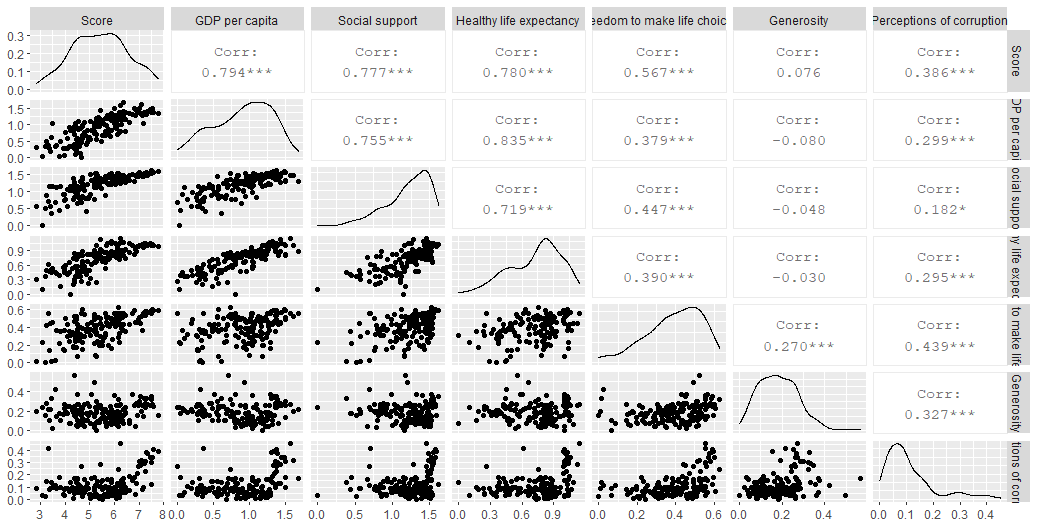
\includegraphics[width=\linewidth]{hap19_pairs.png}
    \caption{Pairwise Scatter Plot of 2019's WHR Data}
    \label{hap19pairs}
\end{figure}

Lastly, it may be interesting to examine the differences in continent or region in the compilation of the happiness score. Table \ref{countries}, at least at the extremes, indicates that European countries are far happier than African countries. Figure \ref{hapbox} displays box plots of the happiness scores by region of the world. Africa has lowest mean happiness, while Australia and New Zealand have the highest median. Europe and the Middle East appear to have the widest distribution of happiness scores. It appears, at least at first glance, like the Region one's country is in may determine the happiness of the country, though this factor is unaccounted for in the WHR.

\begin{figure}[H]
    \centering
    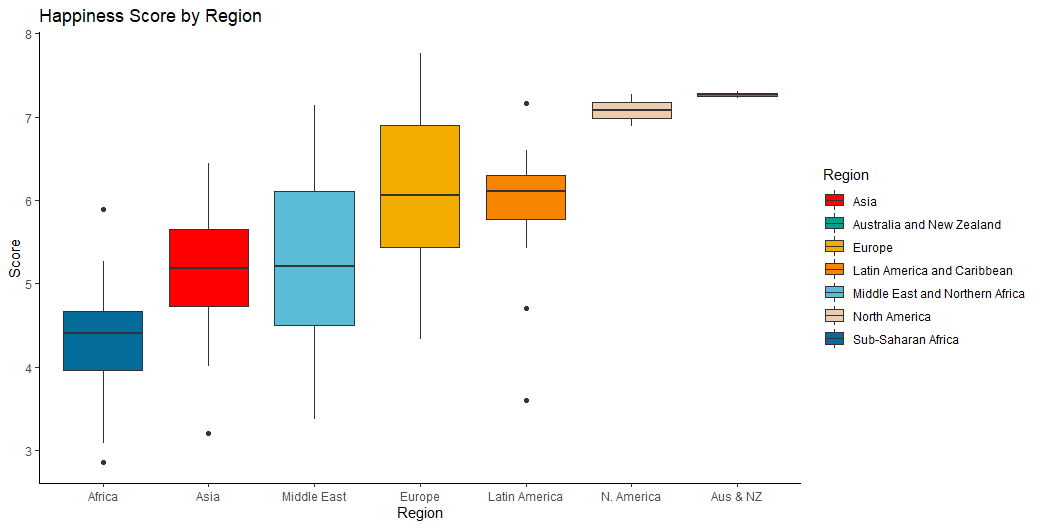
\includegraphics[width=\linewidth]{hap_box.png}
    \caption{Box Plot of Happiness Scores by Region}
    \label{hapbox}
\end{figure}


\section{Happiness on the Straight and Narrow: Simple Regression}
Linear regression is a bread-and-butter tool for examining relationships between independent and dependent variables. In our case, a linear regression model can help us determine if there is a linear relationship between our independent variables and dependent variable, \textit{score}. Additionally, it can help us determine if the effect is statistically significant or just noise, as well as determining the magnitude of said effect.\\\\
\textit{Score} is regressed on all independent variables, resulting in the following equation:
\begin{align*} \hat{Score} = 1.79 + 0.78GDP + 1.12Social + 1.08LifeExp + 1.45Freedom + 0.49Generosity + 0.97Corruption \end{align*}
where a one unit increase of \textit{GDP}, for example, leads to a 0.78 increase in the happiness \textit{score}. The other independent variables can be interpreted in similar ways: a one unit increase in \textit{social} support leads to a 1.12 increase in \textit{score}, and so on. The model has an adjusted R$^2$ of 0.77, meaning it explains about 77\% of the variation in the variable \textit{score}. However, \textit{generosity} and \textit{corruption} are not statistically significant at the 0.05 level, with p-values of 0.32 and 0.07, respectively, while p-values for all other variables are less than 0.01.\\\\
We decided to remove \textit{generosity} and \textit{corruption} from the original model, then refit the regression. The new estimated regression equation becomes:
\begin{align*} \hat{Score} = 1.89 + 0.81GDP + 1.02Social + 1.14LifeExp + 1.85Freedom \end{align*}
where a one-unit increase in \textit{GDP} now leads to a 0.81 increase in \textit{score}, ceteris paribus, and so on. This model has an adjusted R$^2$ of 0.76, meaning it only explains 1\% less of the variance in \textit{score} than the original model, even after excluding two variables. In other words, \textit{generosity} and \textit{corruption} appear to be relatively unimportant in the determination of the happiness \textit{score}.\\\\
It is important to ensure this reduced regression model, which appears to be the best regression model, does not violate any key assumptions, the foremost being homoscedasticity (equal variance) and linear independence (i.e., no multicollinearity). Figure \ref{model_diags} displays a QQ plot of the model's residuals and a scatter plot of the residuals versus the fitted values, the latter containing a line at y=0 for scale. The residuals follow the QQ plot reasonably well, with some deviation along the tails. A Shapiro-Wilk test was performed on these residuals, and it returned a p-value of 0.08, meaning we fail to reject the null hypothesis and conclude our residuals are likely normal, satisfying another key model assumption. Additionally, the residuals appear to be distributed randomly as the fitted values increase, which indicates heteroscedasticity is not a problem. Finally, a Variance-Inflation Factor test was conducted on this regression model, and the highest value returned was 3.96, far less than the commonly accepted threshold of 10. Multicollinearity appears not to be an issue with this regression model. In fact, the model appears well-specified.

\begin{figure}[H]
    \centering
    \subfloat[QQ Plot]{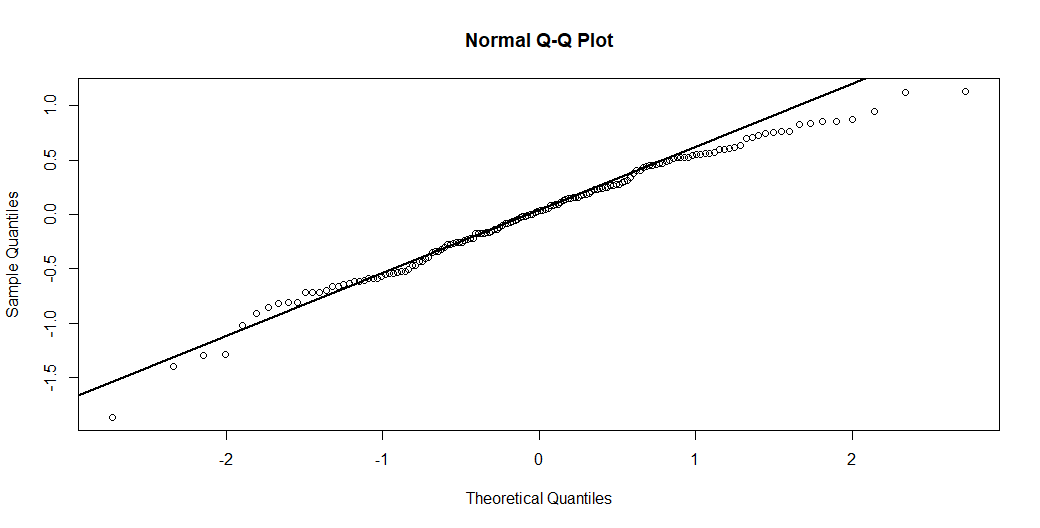
\includegraphics[width=11cm]{reg_qq.png}}\\
    \subfloat[Residuals vs. Fitted Values]{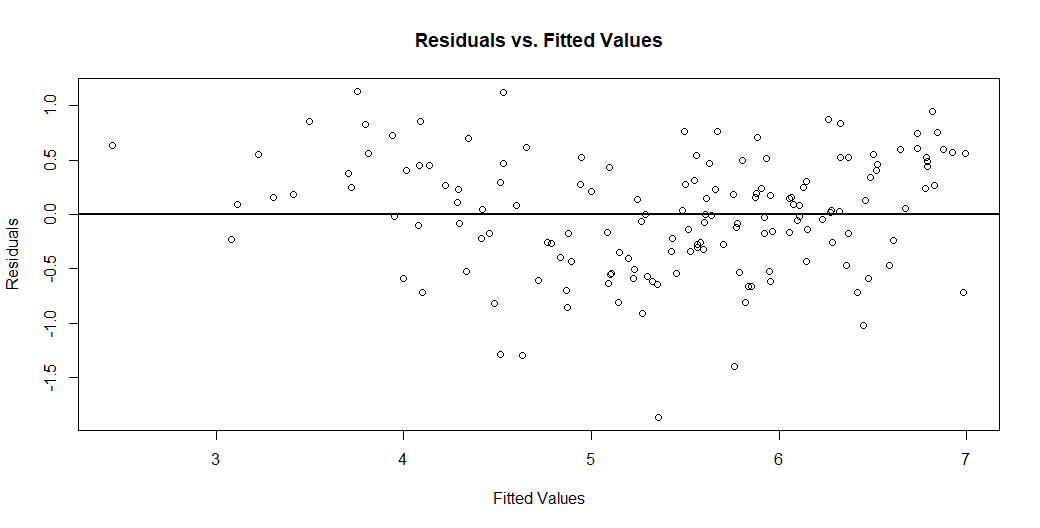
\includegraphics[width=11cm]{reg_resids.png}}
    \caption{Regression Model Diagnostic Plots}
    \label{model_diags}
\end{figure}


\section{Stay Happy, My Friend: Changes over Time}
For our time series analysis, we began by finding the mean value of various measures for each year within a given geographical region.This can be seen in Fig. \ref{fig:series}. From this we can see how the various measure evolve over time. For Rank, we see that all regions saw a significant change in the ranking. 6 of the ten regions saw a decrease in ranking, while 3 of the ten saw an increase in ranking. This is also seen in the scores. In terms of GDP, we see that for all regions, the GDP score is better in 2019 than in 2015, but is actually the best in 2016/2017. For Family, the scores universally bottom out at 2016, but subsequent years are all above 2015. For Health, we see a similar trend, with a drop from 2015 to 2017 followed by a rise to peak values in 2019. For Freedom, we see that the score is erratic, however, there appears a trend of moving back and forth from low freedom score to high freedom score and back. For Trust, we see that the majority have a decreased, with 6 out of 10 regions strictly dropping in trust every year and the remaining 4 out of 10 having decreased overall. For Generosity, we see that all regions have fallen, and that the general behavior across all regions is the same, with a large drop off from 2017 to 2018.\\

\begin{figure}[h]
    \centering
    \subfloat[Rank]{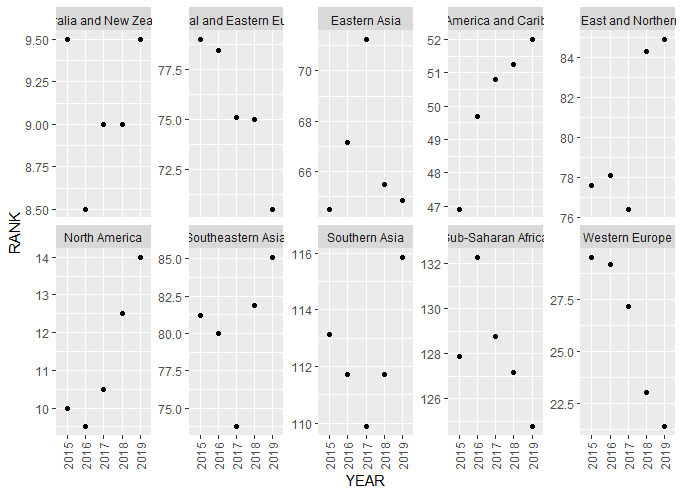
\includegraphics[width=7cm,height=5cm]{Regional_Mean/Rplot8.png}}
    \subfloat[Score]{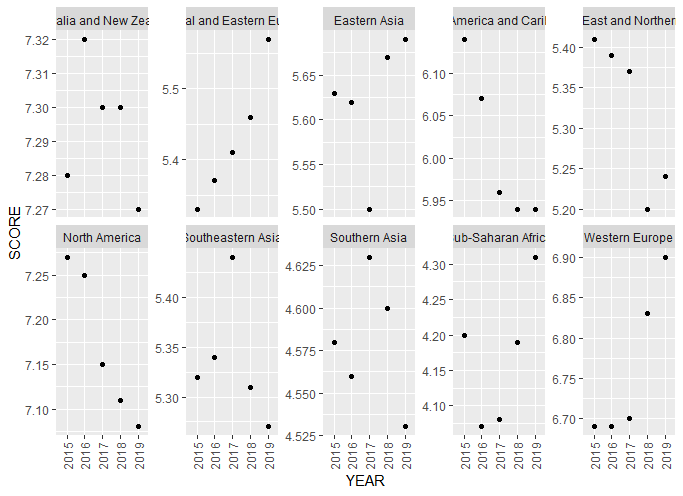
\includegraphics[width=7cm,height=5cm]{Regional_Mean/Rplot7.png}}\\
    \subfloat[GDP]{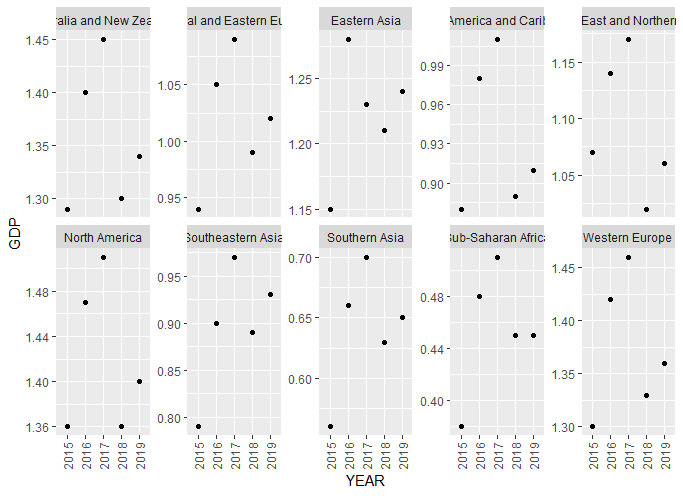
\includegraphics[width=7cm,height=5cm]{Regional_Mean/Rplot6.png}}
    \subfloat[Family]{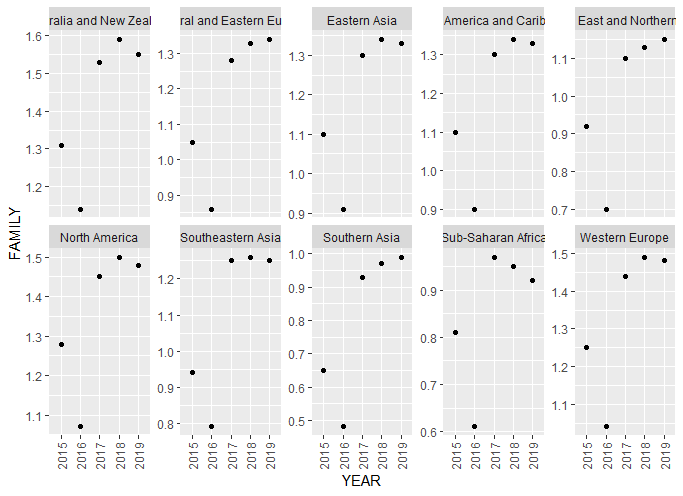
\includegraphics[width=7cm,height=5cm]{Regional_Mean/Rplot5.png}}\\
    \caption{Mean Values per Year per Region}
    \label{fig:series}
\end{figure}

While using only 5 years for analysis does not allow for a great amount of detail, it still allows for some analysis. GDP, Family, Health, Freedom, and Generosity all have similar trends across all regions and they have similar overall trends to the respective regions happiness score. Thus, we may expect Trust to have a larger impact in terms of the differences between regions happiness score. Comparing the Happiness and trust scores, we can see that for some of the regions an increase in trust occurs with an increase in happiness score, but for other the opposite occurs. Thus, we can also conclude that Trust is not a influencing variable on happiness Score as a whole.

\begin{figure}[H]
    \centering
    \subfloat[Health]{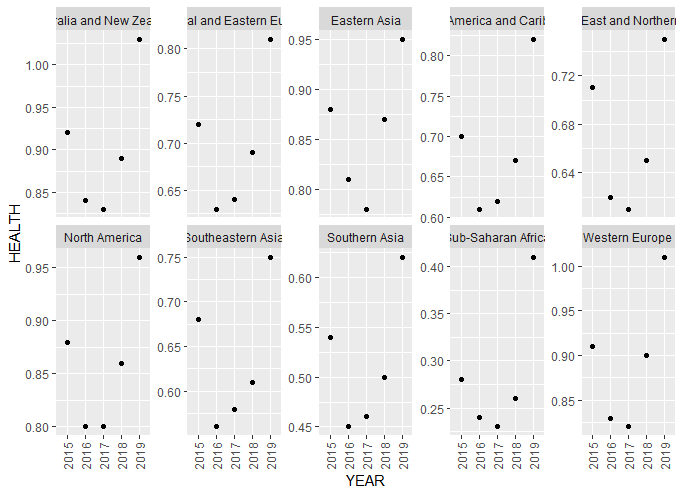
\includegraphics[width=7cm,height=5cm]{Regional_Mean/Rplot4.png}}
    \subfloat[Freedom]{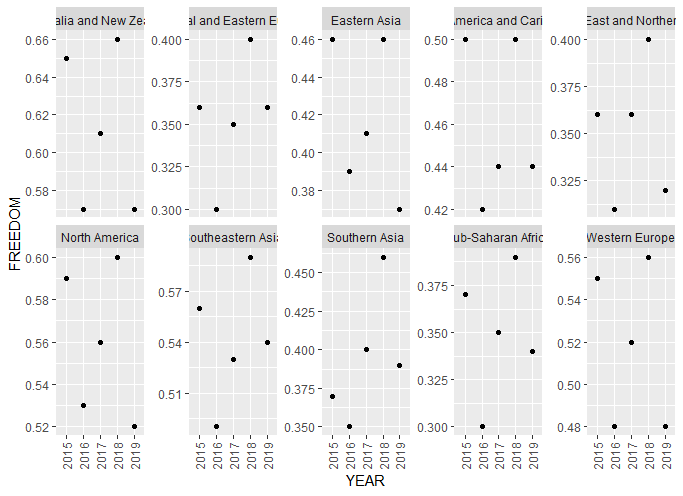
\includegraphics[width=7cm,height=5cm]{Regional_Mean/Rplot3.png}}\\
    \subfloat[Trust]{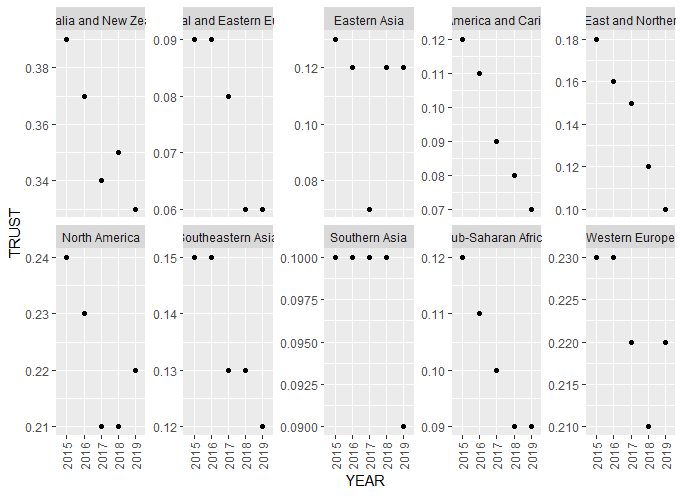
\includegraphics[width=7cm,height=5cm]{Regional_Mean/Rplot2.png}}
    \subfloat[Generosity]{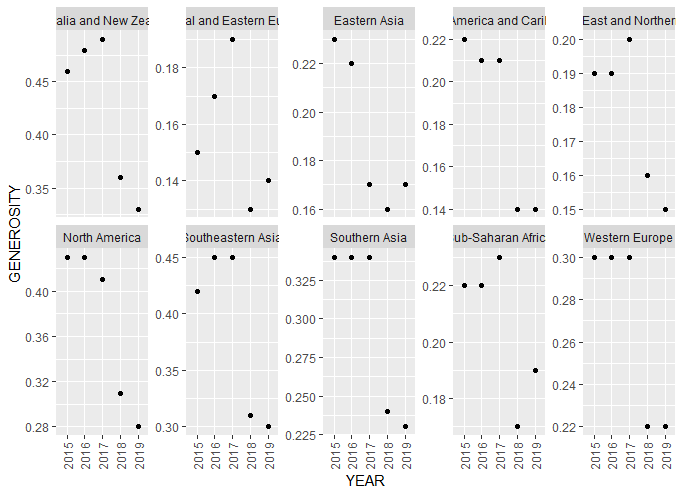
\includegraphics[width=7cm,height=5cm]{Regional_Mean/Rplot1.png}}
    \caption{Mean Values per Year per Region cont.}
    \label{fig:sereis2}
\end{figure}

With these factors in mind we can compare the mean value of the happiness score across all countries for each year with the similar mean values of GDP, Family, Health, Freedom, and Generosity. The results are as in Fig. \ref{fig:time_pred}, which contains plots of the means with 95\% confidence intervals. The creation of the confidence intervals required manipulation of the data, as not all fields were present across all data sets. The 2015 data set contained score and its standard deviation, but not pre-supplied confidence intervals. Thus the intervals where calculated using a confidence level of 95\%. The 2016 and 2017 data sets contained score and intervals, but did not contain the standard error. The standard error was calculated from these, and since the confidence of the intervals is not stated, a 95\% level was assumed. The 2018 and 2019 lacked both standard error and intervals, and so artificial ones were created based on the prior years.\\

This process was accomplished by first taking the ratio of the total mean standard error to the total mean score for each year. The mean of these was taken and then used to scale the total mean score of the 2018 and 2019 to establish an estimated mean for their standard deviations. We justify this approach by noting that the ratio for each year is relatively similar and in addition it utilizes information from the 2018 and 2019, whereas directly using the mean of total mean standard errors from the prior years does not. This is not an airtight method however as the number of data points is very small. The mean of the mean standard errors for each year was found and a normal distribution was created from these to act as the standard errors of the lacking years.

\begin{figure}[H]
    \centering
    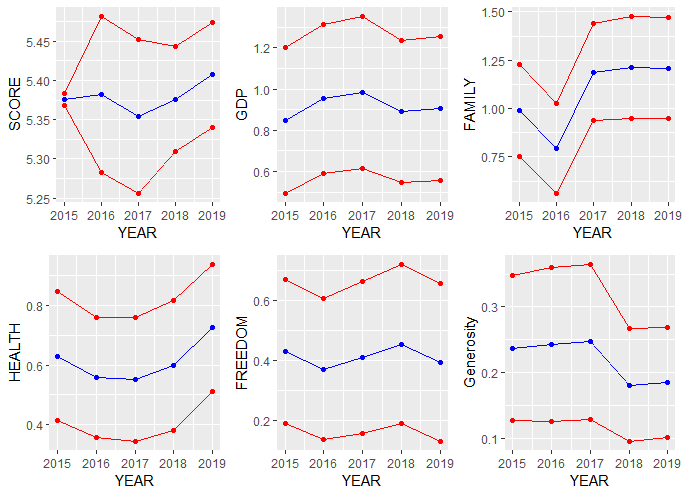
\includegraphics[width=12cm]{Regional_Mean/RplotA.png}
    \caption{Mean values across all countries. Blue lines indicate mean value, Red lines indicate 95\% confidence intervals.}
    \label{fig:time_pred}
\end{figure}

From Fig. \ref{fig:time_pred}, we see that Score and its interval behave weirdly. The distance of the interval in 2015 is incredibly small,while the distance for 2016 and 2017, though roughly trending the same as the mean score, are very wide. The interval at 2018 and 2019 shows the best behavior, which may be due to the fact it was calculated using means of means. Further examination of the figure shows us that Family has the largest difference in behavior from the happiness score, thus we may wish to focus less on it when deciding on a model. From Figure \ref{fig:ERR}, we see that the standard error of the happiness score has similar strange behavior as did the mean. We can conclude from this and the above figure that the most change occurred between 2015 and 2016.

\begin{figure}[h]
    \centering
    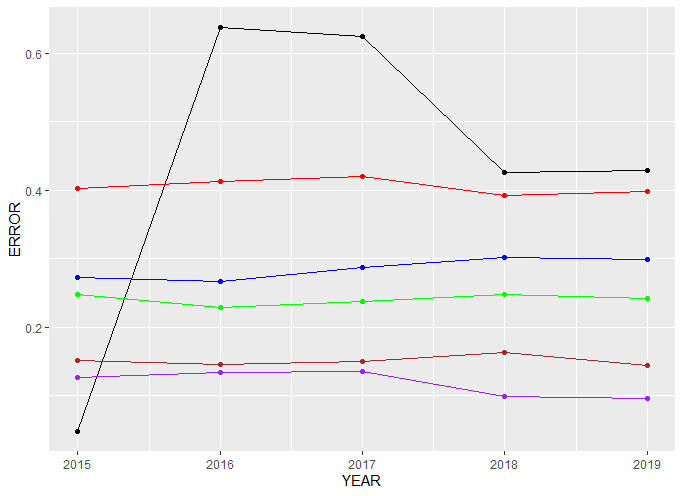
\includegraphics[width=11cm,height=6cm]{Regional_Mean/RplotB.png}
    \caption{Standard Errors of variables. From top to bottom: Score, GDP, Family, Health, Freedom, ans Generosity}
    \label{fig:ERR}
\end{figure}

\newpage

\section{Throw away Your Books on Tape: Simplifying Happiness}
In a recent New Yorker article called, "What Data Can't Do," Hannah Fry, a professor of spatial statistics at University College in London, revisited the "fragile family" study done by researchers at the start of the millenium. In the study, researchers tracked thousands of families with newborns over a long period of time, eventually collecting about thirteen thousand data points on each individual child. Then, instead of releasing their findings on how the children ended up (their educational performance, presence of behavioral problems, etc.), the researchers invited scientists around the world to make predictions using any machine learning model they pleased. The researchers posed a very simple model as a baseline: predicting a future child's performance by just four data points, three of which were available at the child's birth. The simple model explained 20\% of the variance in the children's GPAs, while the most sophisticated ML model, with access to the data's entire 13,000 features, only explained 23\%. Fry writes the researchers observed that statistical models are "better at predicting each other" than predicting reality.\\\\
Likewise, the WHR is a fascinating experiment in data aggregation and the methodology of ratings, but we were curious: what happens when this complicated model becomes very simple? Is the decrease in performance that drastic? Does the model only explain 20\% of variance instead of 23\%? And does it matter?\\\\
To begin to answer these questions, we took the most recent life expectancy data from the World Bank (available in 2018), and ran a very simple regression using it as the predictor for the 2019 happiness \textit{score}. The thinking is, one will be satisfied with their life if they know they can expect much of it.\\\\
The estimated regression equation becomes
\begin{align*}
    \hat{Score} = -2.41 + 0.11LifeExp
\end{align*}
where \textit{Score} is the predicted 2019 happiness \textit{score} and \textit{lifeexp} is the average life expectancy in years for the resident of a particular country. Every additional year in life expectancy leads to a 0.11 increase in the happiness \textit{score}. Both the intercept and slope parameter are significant at the 0.001 level, and this model explains 57.8\% of the variation across \textit{score}. \\\\
According to the Shapiro-Wilk test, the simple model's residuals are not, strictly speaking (strictness here meaning our paper-wide significance level of 0.05) normal, returning a p-value of the devastatingly close 0.04. However, plotting the qq plot and the residuals versus the fitted values in Figure \ref{simp_resids} shows only a slight deviation in the upper tail of the residuals, and the scatter plot yields no apparent pattern in these residuals as the fitted values increase. Further, we almost expect our simple model of \textit{lifeexp} to fail to explain the happiness \texit{score} completely, so the fact that we do not observe patterned or obviously abnormal residuals is cause for celebration, not concern. We can proceed to comparing the simple and complex models.\\\\
The ideal regression model from the World Happiness Report (as explained in Section 3) explains 76\% of the variance in the happiness score, while our simple life expectancy model explains only 57.8\%. This is already a sign that the ideal regression model likely significantly outperforms the simple life expectancy model. A more rigorous analysis of variance (anova) test was conducted to compare these two models, and the models are substantially different, with an F-statistic of 41.7 and corresponding p-value near 0. The mean squared error (MSE) of the life expectancy model is 0.52, while the MSE of the ideal WHR model is a much smaller 0.28. This means we can expect the average error of the simple model to be 0.52 happiness points, while the average error of the WHR model is only 0.28 happiness points. In every metric, the ideal WHR model is better. It turns out, those three extra variables - \textit{GDP per capita, social support}, and \textit{freedom} - are essential to explaining the happiness \textit{score}.

\begin{figure}[h]
    \centering
    \subfloat[QQ Plot]{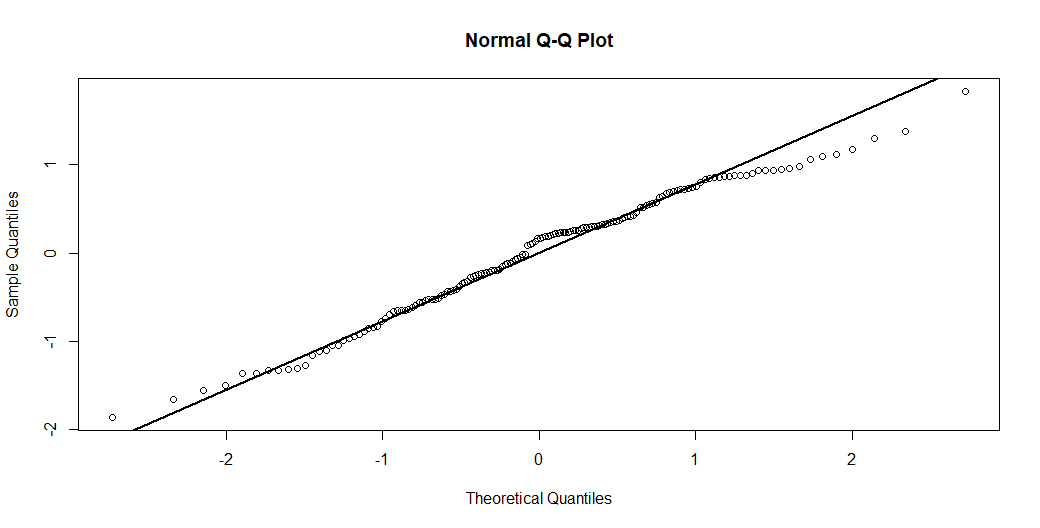
\includegraphics[width=11cm]{simp_qq.png}}\\
    \subfloat[Residuals vs. Fitted Values]{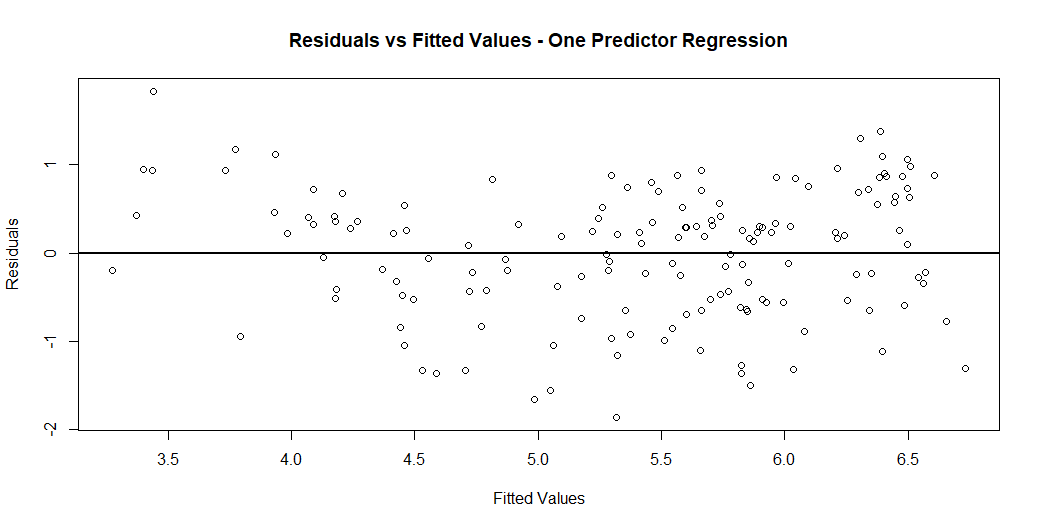
\includegraphics[width=11cm]{simp_resids.png}}
    \caption{Life Expectancy Model Diagnostic Plots}
    \label{simp_resids}
\end{figure}

\section{Happiness \textit{Is} a Butterfly: An Elusive Conclusion}
Along with the World Happiness Report, this paper has shown us a few things. One, that western European countries are the happiest, and have been the happiest since the inception of the report. Two, that a country's economy, social support, life expectancy, and general freedoms are indispensable for a citizenry's happiness. Three, that war-torn countries are the least happy, as economic activity, social goodwill, a high life expectancy, and liberty are not qualities one typically finds on a battlefield. \\\\
While this paper has performed standard statistical analysis on the data provided, your humble authors still cannot shake the feeling that the World Happiness Report is, in a word, shoddy. Its methods keep evolving, its data transformations and aggregations are opaque, yet somehow, the happiest countries remain the ones in which the authors reside. Though we do not dispute the fact that happiness is likely elusive in, for example, Yemen, it seems audacious to present an authoritative ranking of happiness when generations of philosophers, scientists, and theologians still aren't even sure what happiness is. \\\\
At least the World Happiness Report is good for a few days of New York Times articles, which is reward enough for us all.

\end{document}